\documentclass[12pt]{article}
\usepackage[utf8]{inputenc}
\usepackage[T1]{fontenc}
\usepackage{lmodern}
\usepackage{graphicx}
\usepackage{subcaption}

\usepackage[svgnames]{xcolor}
\usepackage[a4paper,bindingoffset=0.2in,%
            left=0.5in,right=0.5in,top=0.5in,bottom=1in,%
            footskip=.25in]{geometry}
\pagenumbering{gobble}
\usepackage[colorlinks=true, linkcolor=Black, urlcolor=Blue]{hyperref}


\begin{document}
	\title{Sprawozdanie - Odtwarzanie muzyki z nut na pięciolinii}
	\author{Marcin Zatorski 136834, Sebastian Michoń 136770}
	\date{\vspace{-2ex}}
	\maketitle
	\section{Cel i zakres projektu}
	Celem projektu było zaimplementowanie aplikacji odpowiedzialnej za odczytywanie nut z pięciolinii za pomocą kamery, a następnie odtwarzanie ich za pomocą głośnika z użyciem płytki rapsberry pi.
	\section{Schemat}
	\begin{enumerate}
		\item \underline{Idea, połączenie, schemat - będą zdjęcia}
	\end{enumerate}
	
	\section{Projekt a realizacja}
	\begin{enumerate}
		\item Założeniem projektu była implementacja kodu, który odczytuje nuty z kamery ze skutecznością nie mniejszą niż 65\%, który nie będzie funkcjonował wiele wolniej niż kod języka C++, który będzie odtwarzał dźwięk zadany nutami na głośniku.
		\item Założenie zostało zrealizowane - aplikacja osiąga skuteczność dochodzącą do 90\% przy poprawnym oświetleniu i odpowiednio bliskim ustawieniu kamery, ponadto pomimo implementacji kodu w języku Python kluczowe jego sekcje zostały przepisane do Cythona, co przyspieszyło aplikację o ponad 2000\% i umożliwiło jej uruchamianie na płytce rapsberry pi.
		\item Projekt można rozwinąć głównie przez porzucenie metod analitycznych przy konstrukcji heurystyk wykrywających nuty na zdjęciu na rzecz wytrenowanych konwolucyjnych sieci neuronowych albo innych technik, których działania nie da się aproksymować (np. Light Gradient Boosting Machine). Poza tym można przepisać mniej kluczowe części kodu do języka Cython, co dodatkowo zmniejszy czas potrzebny na odtworzenie dźwięku.
	\end{enumerate}

	\section{Kluczowe fragmenty kodu}
	\begin{enumerate}
		\item \underline{Które kody - integracja czy analiza nut? Dopiszę tu swoją część cythona, przynajmniej interfejsy}
		\item \underline{Pewnie także integracja z pythonem}
	\end{enumerate}

	\clearpage
	\section{Zdjęcia fizycznych połączeń urządzeń}
	\begin{figure}[h!]
		\centering
		\begin{subfigure}[b]{0.32\linewidth}
			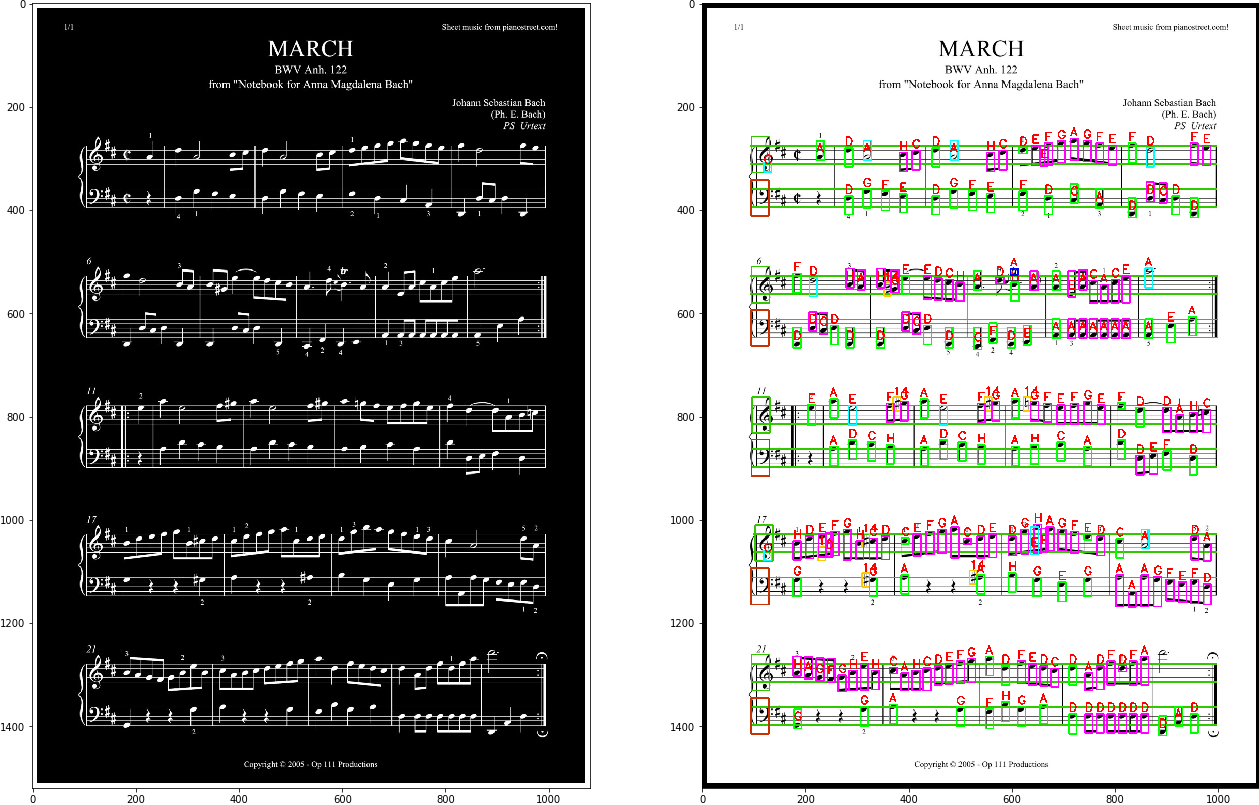
\includegraphics[width=\linewidth]{zdjs/Zdj0.png}
			\caption{Pierwszy podpis}
		\end{subfigure}
		\begin{subfigure}[b]{0.32\linewidth}
			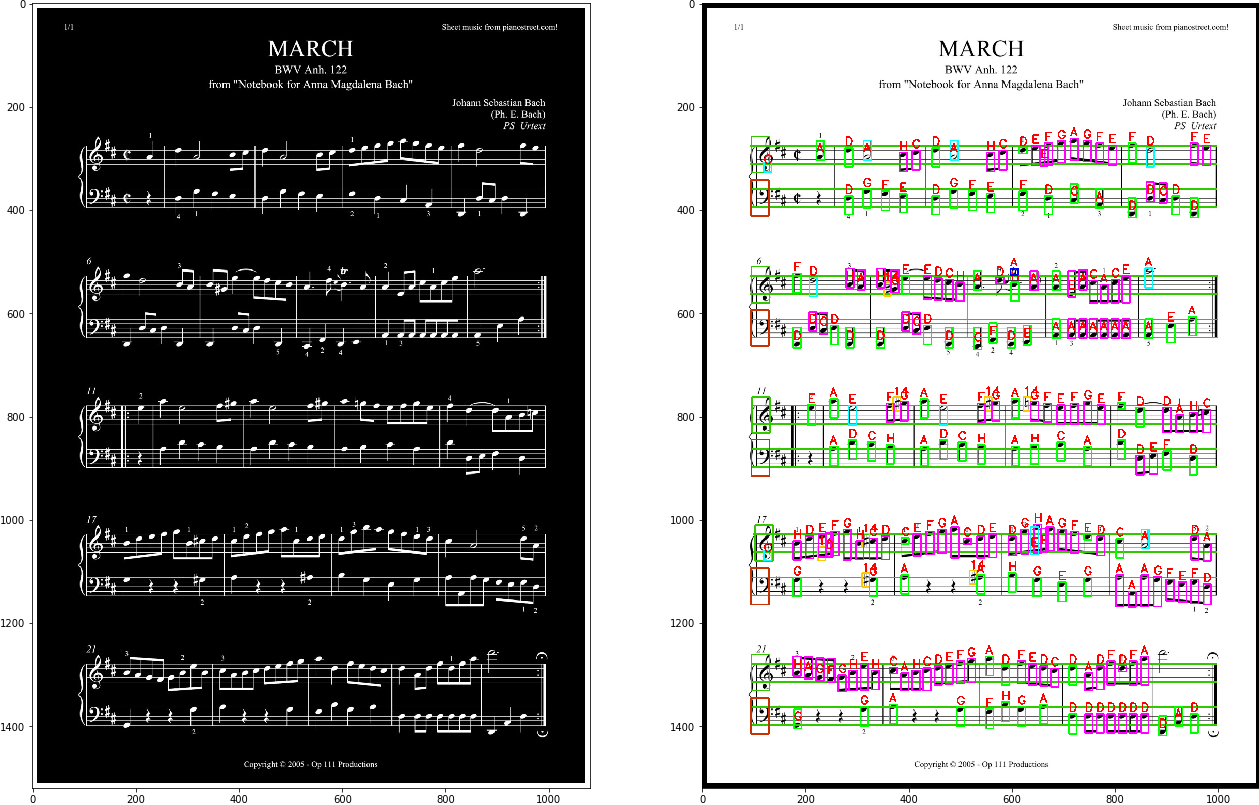
\includegraphics[width=\linewidth]{zdjs/Zdj0.png}
			\caption{Drugi podpis}
		\end{subfigure}
		\begin{subfigure}[b]{0.32\linewidth}
			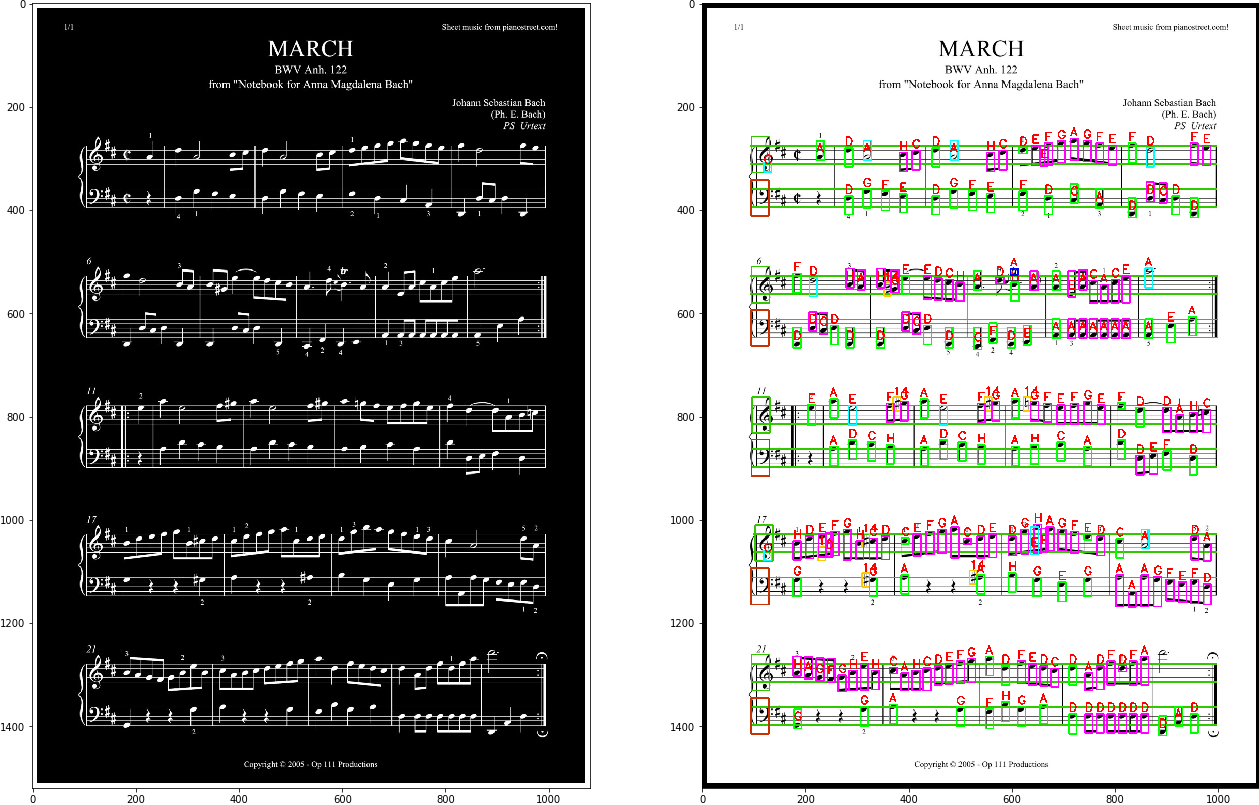
\includegraphics[width=\linewidth]{zdjs/Zdj0.png}
			\caption{Trzeci podpis}
		\end{subfigure}
	
		\begin{subfigure}[b]{0.48\linewidth}
			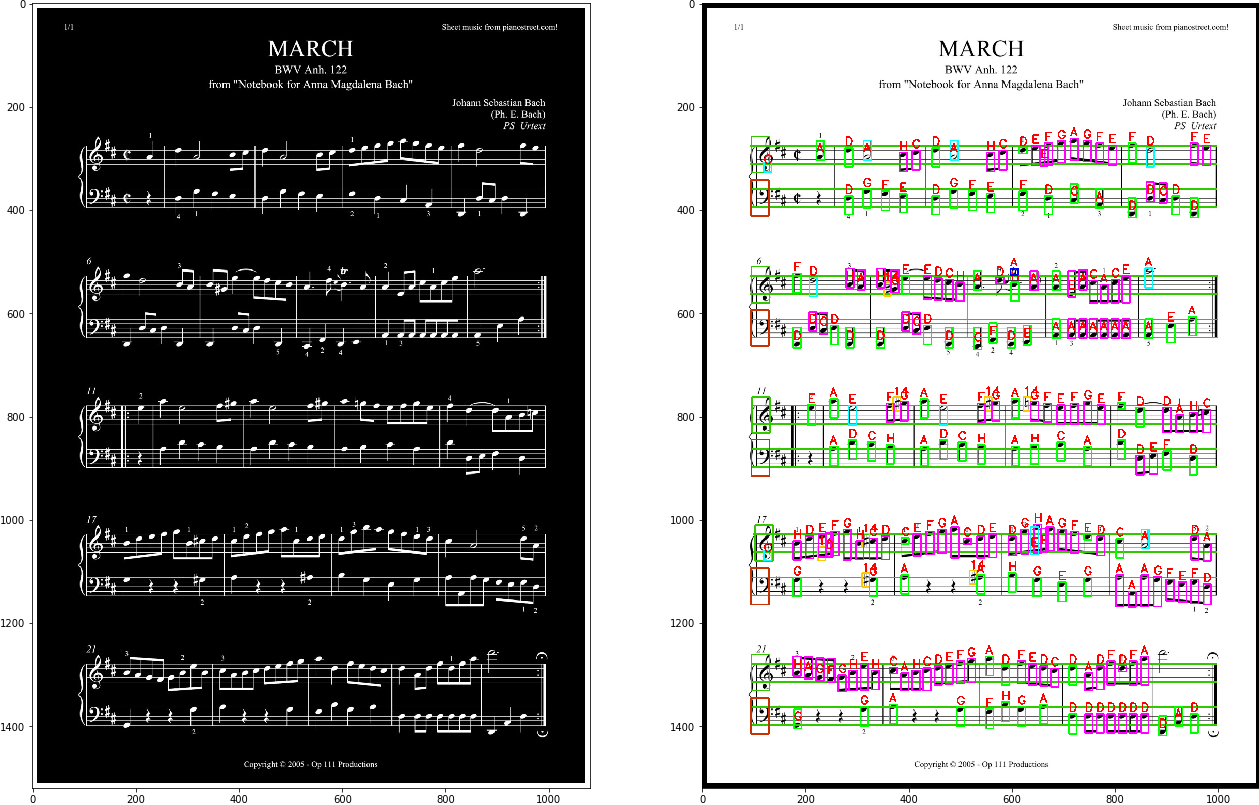
\includegraphics[width=\linewidth]{zdjs/Zdj0.png}
			\caption{Czwarty podpis}
		\end{subfigure}
		\begin{subfigure}[b]{0.48\linewidth}
			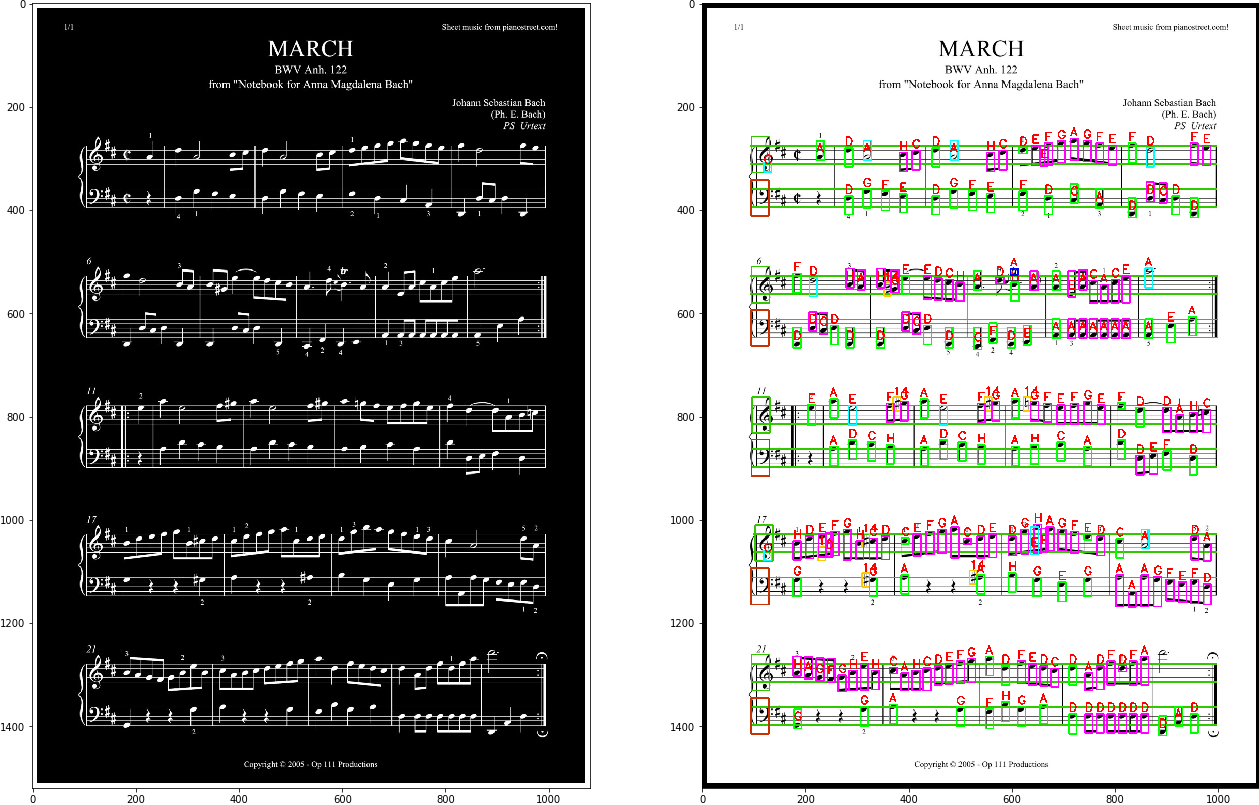
\includegraphics[width=\linewidth]{zdjs/Zdj0.png}
			\caption{Piąty podpis}
	\end{subfigure}
	\end{figure}

	\section{Podsumowanie, wnioski}
	\begin{enumerate}
		\item Aplikacja realizuje swój cel, choć pewne elementy niezwiązane z systemami wbudowanymi możnaby wykonać lepiej.
		\item Kod zaimplementowany przez nas uzyskuje wysoką skuteczność przy korzystnej scenie zdjęcia; zasadnym zdawałoby się rozpocząć próbę ulepszenia tego kodu od użycia metod adaptatywnych, opartych na funkcji kosztu zamiast metod analitycznych przetwarzania obrazu.
	\end{enumerate}

\end{document}
